\documentclass[a4paper,12pt]{article}
\usepackage{tikz}
\usetikzlibrary{calc}
\begin{document}

%\begin{center}
%\begin{tikzpicture}
%
%	\foreach \i [remember=\i as \j (initially 0), evaluate=\i as \c using 100*\i/100] in {10,20,...,100} {
%		%\fill [yellow!\c](\j:0.5) circle (0.5);
%		\fill [red!\c](\i:1) circle (0.5);
%		%\fill [blue!\c](-\j:0.5) circle (0.5);
%		\fill [black!\c](-\i:1) circle (0.5);
%	}
%\end{tikzpicture}
%\end{center}
%\begin{figure}
%%\centering
%\begin{tikzpicture}[line width=0.8pt]
%\foreach \i in {-9,...,9}{
%	\foreach \j in {-9,...,9}{
%		\coordinate(v\i\j) at (\i,\j);
%		\foreach \k in {1,...,8}{
%			\coordinate(v\i\j\k) at ($(v\i\j)+(\k*45-22.5: 0.3)$);
%		}
%	}
%}
%
%\draw (v02)--(v04)--(v26)--(v46)node[near start, above]{$a$}--(v64)--(v62)node[near end, right]{$a^{-1}$}--(v40)--(v20)--cycle;
%
%\draw [dashed](v33)--(v11);
%\draw [dashed](v33)--(v03);
%\draw [dashed](v33)--(v15);
%\draw [dashed, ->](v33)--(v37);
%\draw [dashed](v33)--(v55);
%\draw [dashed](v33)--(v63);
%\draw [dashed, ->](v73)--(v63);
%\draw [dashed](v33)--(v51);
%\draw [dashed](v33)--(v30);
%
%\draw [dashed, ->](v33)--(v30);
%
%
%\end{tikzpicture}
%\end{figure}

\begin{figure}
\centering
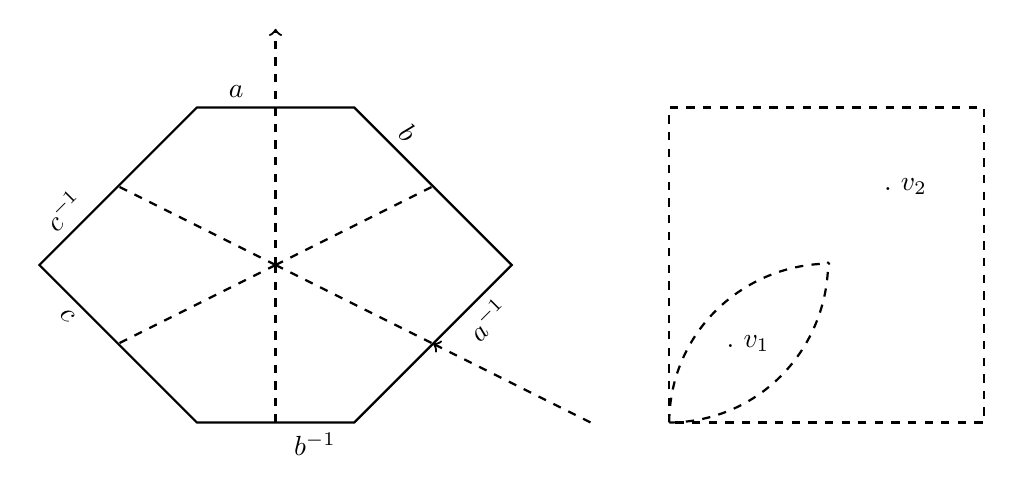
\begin{tikzpicture}[line width=0.8pt]
\foreach \i in {-9,...,9}{
	\foreach \j in {-9,...,9}{
		\coordinate(v\i\j) at (\i,\j);
		\foreach \k in {1,...,8}{
			\coordinate(v\i\j\k) at ($(v\i\j)+(\k*45-22.5: 0.3)$);
		}
	}
}

\draw (v-10)--(v-32)node[near end, sloped,below]{$c$}--(v-14)node[near start, sloped, above]{$c^{-1}$}--(v14)node[near start, above]{$a$}--(v32)node[near start, sloped, above]{$b$}--(v10)node[near start, sloped, below]{$a^{-1}$}--cycle node[near start, below]{$b^{-1}$};


\draw [dashed](v02)--(v-21);
\draw [dashed](v02)--(v-23);
\draw [dashed](v02)--(v21);
\draw [dashed](v02)--(v23);
\draw [dashed](v02)--(v00);
\draw [dashed, ->](v02)--(v05);
\draw [dashed, ->,](v40)--(v21);

\draw [dashed] (v50)--(v54)--(v94)--(v90)--cycle;
\draw [dashed] (v50) arc (180:135:2) arc (135:90:2.06);
\draw [dashed] (v50) arc (270:315:2) arc (315:360:2.06);

\draw (v61) node{$.~v_1$};
\draw (v83) node{$.~v_2$};
\end{tikzpicture}
\end{figure}




\end{document}

